\section{付録のタイトル}
\label{sec:appendix_a}
% \addcontentsline{toc}{section}{\appendixname} % 付録が目次に表示されない場合に使用

これは付録の例である.
付録の表記は「付録A,付録B,付録C,...」のように表示され,図表の番号は「A1, A2, A3, ...」(付録のアルファベット+付録内の通し番号)と表示される.

付録が一つのみである場合,「付録A,付録B,付録C,...」のように分ける必要はない.
この場合,\verb|\section|を\verb|\section*|に書き換えると良い.
付録が目次に表示されなくなった場合,\verb|\addcontentsline{toc}{section}{\appendixname}|を用いる.
図表の番号は,\verb|\renewcommand{\thefigure}{\Alph{figure}}|のようにすると,「Fig.~A, Fig.~B, Fig.~C, ...」と表示される.

\begin{figure}
  \centering
  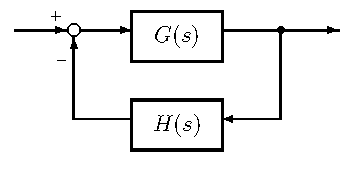
\includegraphics[width=0.6\textwidth]{fig/example.pdf}
  \caption{Figure in the appendix.
    This is an example of a very long caption.
    \lipsum[1]}
  \label{fig:appendix}
\end{figure}

\begin{table}
  \centering
  \caption{Table in the appendix.}
  \label{tab:appendix}
  \begin{tabular}{lrr}
    \hline
    Item   & Price (yen) & Number \\
    \hline
    Apple  & 125         & 5      \\
    Orange & 90          & 10     \\
    Grape  & 320         & 3      \\
    \hline
  \end{tabular}
\end{table}

% 改ページ
\clearpage
